\documentclass[t,8pt]{beamer}

%%% packages
\geometry{paperwidth=140mm,paperheight=105mm}
\usefonttheme[onlymath]{serif}

\usepackage{kotex,amsmath,tabto,setspace,tikz}

\usepackage{tabularx}
%X is not not centered, text moded
\newcolumntype{Y}{>{\centering\arraybackslash}X} % centered, text-moded
\newcolumntype{M}{>{$}X<{$}} % math-moded
\newcolumntype{N}{>{$}Y<{$}} %centered and math-moded
\setlength\tabcolsep{1pt}


%%% counters, commands, environments
\newcounter{num}
\resetcounteronoverlays{num}

\newenvironment{defi}[1]{\refstepcounter{num}\begin{block}{정의 \arabic{num}#1}}{\end{block}}
\newenvironment{theo}[1]{\refstepcounter{num}\begin{block}{정리 \arabic{num}#1}}{\end{block}}
\newenvironment{prob}[1]{\refstepcounter{num}\begin{block}{문제 \arabic{num}#1}}{\end{block}}
\newenvironment{exam}[1]{\refstepcounter{num}\begin{block}{예시 \arabic{num}#1}}{\end{block}}

\newcommand{\pb}[1]%\Phantom + fBox
{\fbox{\phantom{\ensuremath{#1}}}}
\newcommand{\rb}[2]%\Red+fBox
{\fbox{\uncover<#1>{\red{\ensuremath{#2}}}}}
\renewcommand{\arraystretch}{1.5}
\newcommand{\red}[1]{\color{red}{#1}}
\newcommand{\ivs}{\centering\strut\vspace*{-\baselineskip}\newline}%image vertical setting
\newcommand*\circled[1]{\tikz[baseline=(char.base)]{\node[shape=circle,draw,inner sep=2pt] (char) {#1};}}

%%% title
\title{확률과 통계 : 07 연속확률분포}
\institute[ibedu]{아이비에듀}
\date{\today}

%%% toc
\AtBeginSection[]
{\begin{frame}
    \frametitle{목차}
    \tableofcontents[currentsection]
  \end{frame}}


\begin{document}
%%
\frame{\titlepage}

%%%%
\section{연속확률분포}

%%%
\subsection{이산확률분포(복습)}
%%
\begin{frame}[t]{\subsecname}
동전을 두 번 던졌을 때, 앞면이 나온 횟수를 \(X\)라고 하자.
\begin{enumerate}[(1)]
\item
가능한 \(X\)의 값은
\[X=\rb{2-}0,\:\:\rb{2-}1,\:\:\rb{2-}2\]
이다.
따라서 \(X\)는 ({\color<2->{red}{이산확률변수}}, 연속확률변수)이다.
\item<3->
가능한 각각의 \(X\)값에 대하여, 확률을 계산해볼 수 있다 ; 
\begin{align*}
P(X=\textcolor{teal}0)&=_2C_0\left(\frac12\right)^0\left(\frac12\right)^2=\color{teal}{\frac14}\\
P(X=\textcolor{teal}1)&=_2C_1\left(\frac12\right)^1\left(\frac12\right)^1=\color{teal}{\frac12}\\
P(X=\textcolor{teal}2)&=_2C_2\left(\frac12\right)^2\left(\frac12\right)^0=\color{teal}{\frac14}
\end{align*}
이렇게, \(0\)을 넣으면 \(\frac14\)가 나오고, \(1\)을 넣으면 \(\frac12\)가 나오고, \(2\)를 넣으면 \(\frac14\)가 나오는 함수 \(P(X=x)\)를 생각할 수 있다.
이 함수를 \rb{4-}{\text{확률질량함수}}라고 부른다.
\item<5->
확률질량함수는 다음과 같이 표로 나타낼 수도 있고, 그래프로 나타낼 수도 있다.
\begin{minipage}{.46\textwidth}
\begin{tabularx}{\textwidth}{|N|@{}N@{}|@{}N@{}|@{}N@{}|}
\hline
X 		&0		&1		&2\\\hline
P(X=x)	&\frac14	&\frac12	&\frac14\\\hline
\end{tabularx}
\end{minipage}
\begin{minipage}{.46\textwidth}
\centering
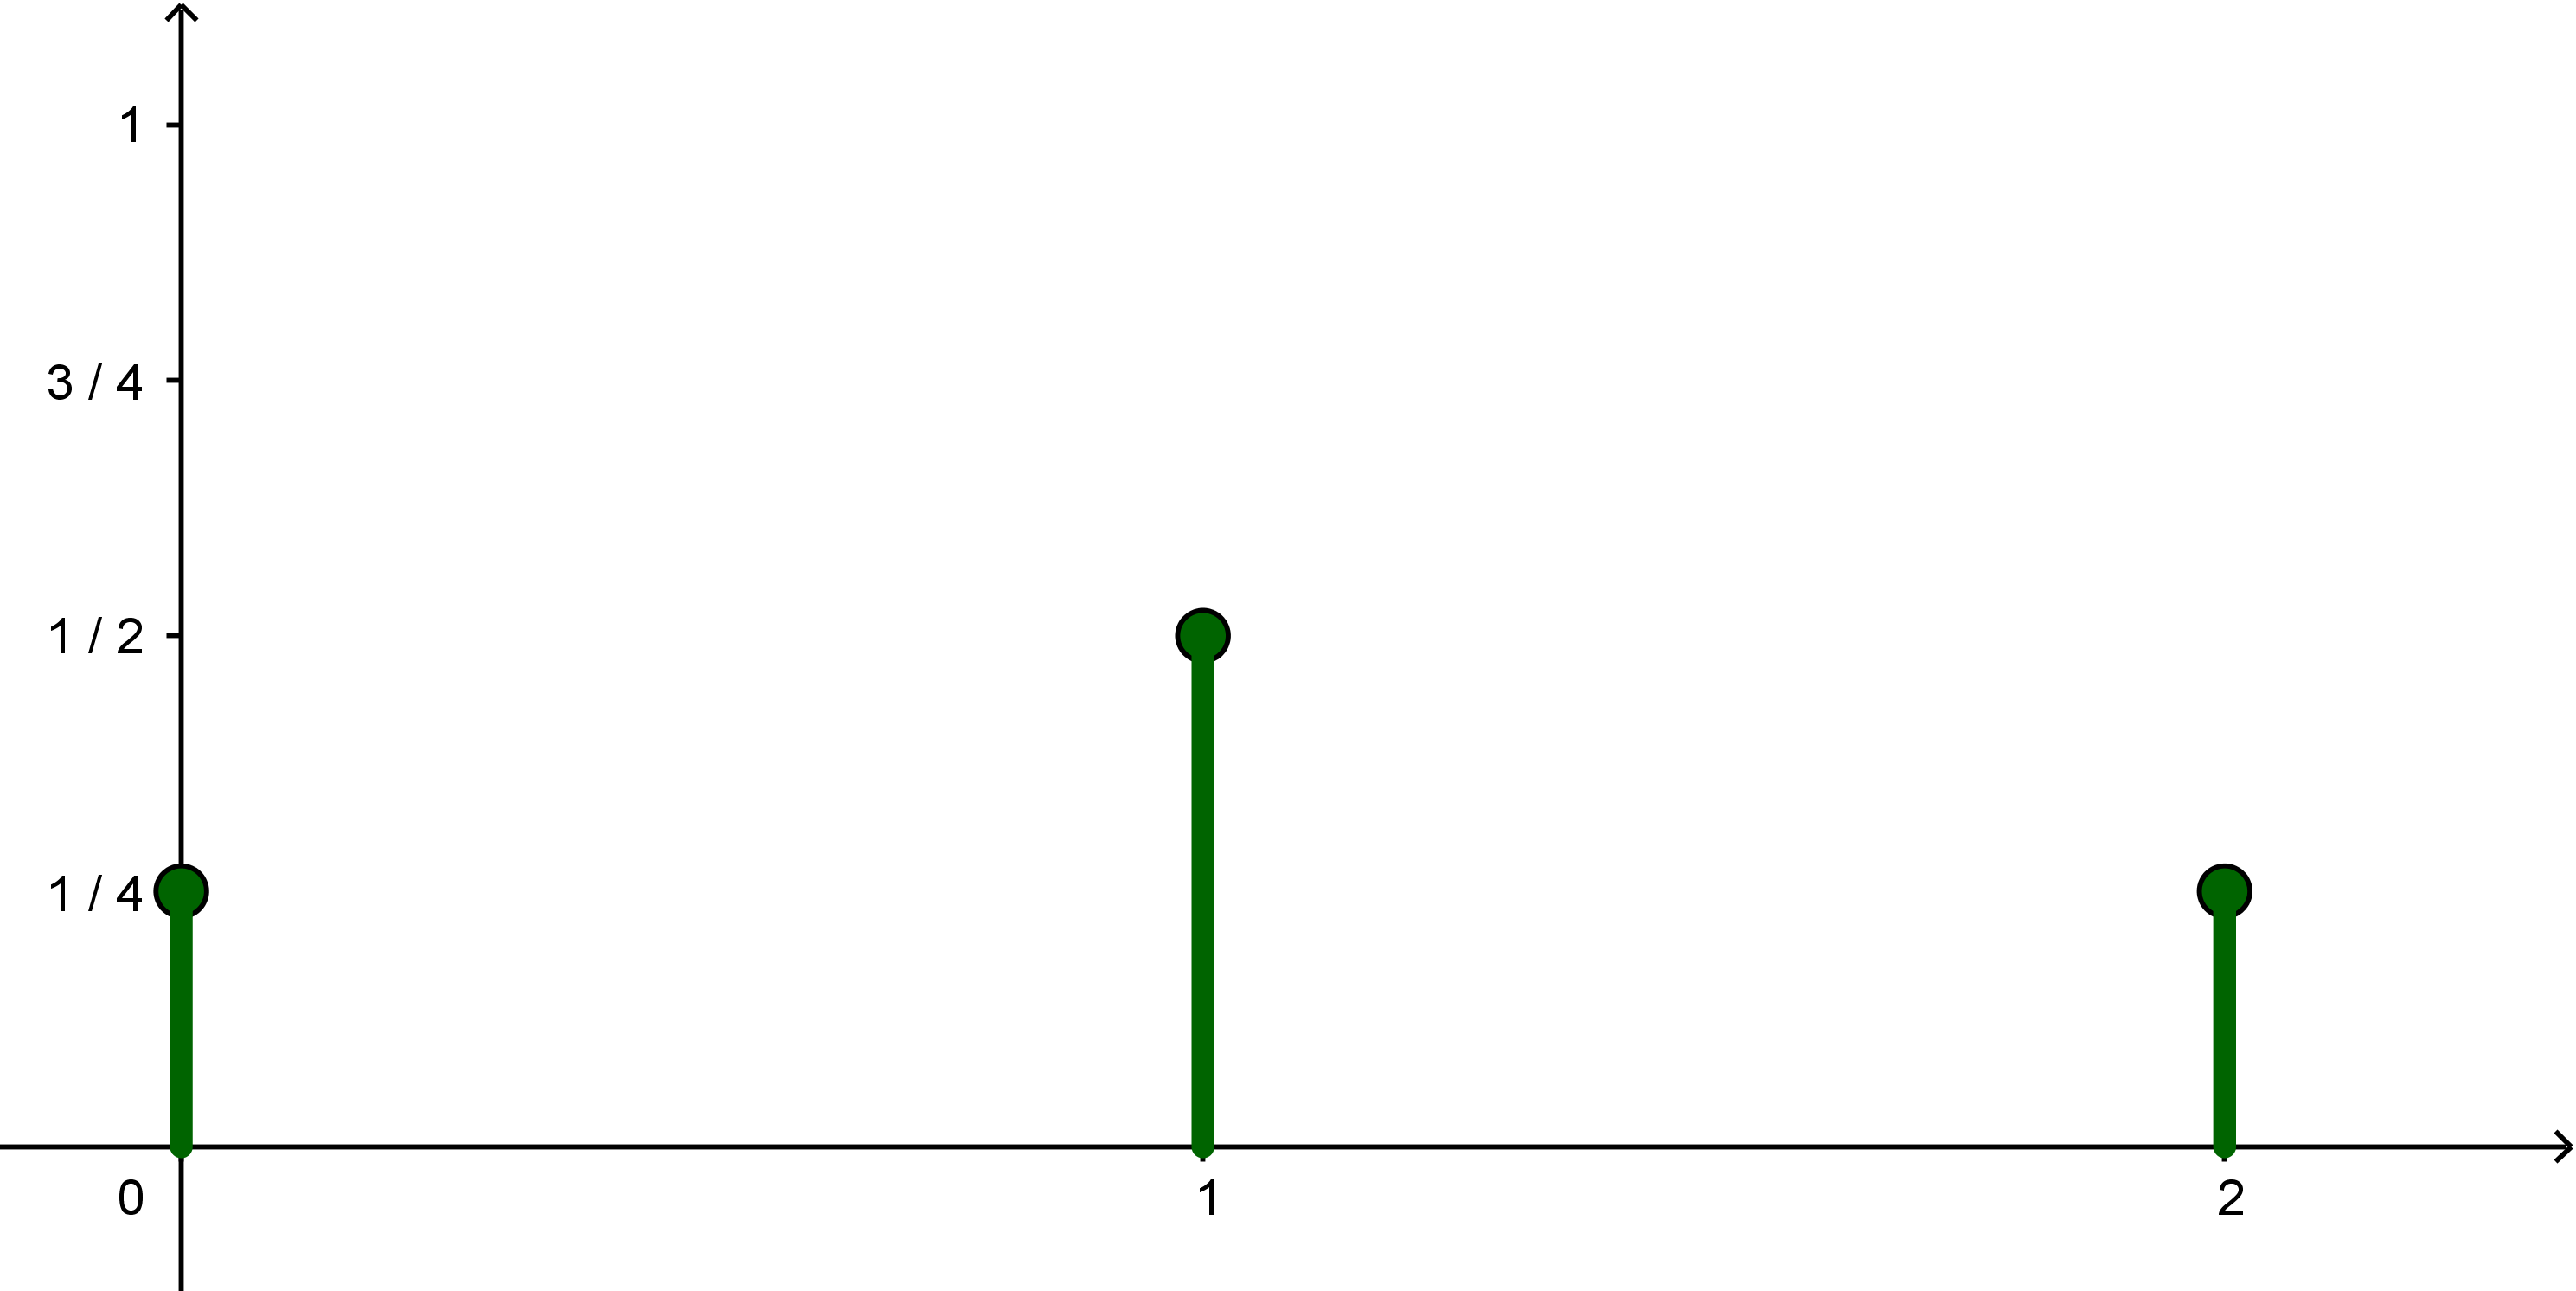
\includegraphics[width=.6\textwidth]{img/1-1}
\end{minipage}
이 표를 \rb{6-}{\text{확률분포표}}라고 하고, 이 그래프를 \rb{6-}{\text{히스토그램}}이라고 부른다.
\end{enumerate}
\end{frame}

%%
\begin{frame}[t]{\subsecname}
\begin{enumerate}[(1)]
\setcounter{enumi}3
\item
이 확률분포에 대한 기댓값과 분산, 표준편차는 다음과 같이 계산한다.
\begin{align*}
E(X)			&=0\times\frac14+1\times\frac12+2\times\frac14=1\\
V(X)			&=E((X-m)^2)=(0-1)^2\times\frac14+(1-1)^2\times\frac12+(2-0)^2\times\frac14=\frac12\\
\sigma(X)	&=\sqrt{V(X)}=\frac{\sqrt2}2.
\end{align*}
\pause
분산을 구할 때에는 \(V(X)=E(X^2)-E(X)^2\)을 활용하여 구해도 된다.
\begin{align*}
E(X^2)		&=0^2\times\frac14+1^2\times\frac12+2^2\times\frac14=\frac32\\
V(X)			&=E(X^2)-E(X)^2=\frac32-1=\frac12
\end{align*}
\item<3->
한편, \(X\)는 사실 \rb{4}{\text{이항분포}}를 따른다고 볼 수 있다.
즉 \(X\sim B(2,\frac12)\)이다.
\uncover<4>{
따라서
\begin{align*}
E(X)		&=2\times\frac12=1\\
V(X)		&=2\times\frac12\times\frac12=\frac12.
\end{align*}}
\end{enumerate}
\end{frame}

%%%
\subsection{연속확률분포}

%%
\begin{frame}[t]{\subsecname}
오른쪽 그림과 같이 세 점 \(A(0,0)\), \(B(2,0)\), \(C(2,2)\)으로 이루어진 삼각형 \(ABC\)가 있다.
이 삼각형의 내부에 임의로 한 점 \(Q\)를 잡을 때, \(Q\)의 \(x\)좌표를 \(X\)라고 하자.
\begin{minipage}{.66\textwidth}
\begin{enumerate}[(1)]
\item
이 삼각형의 넓이는 \rb{2-}{2}이다.
\item<2->
가능한 \(X\)의 값의 범위는 \rb{3-}{0\le X\le 2}이다.\\[5pt]
따라서 \(X\)는 (이산확률변수, {\color<3->{red}{연속확률변수}})이다.
\item<4->
\(P(0\le X\le1)=\rb{5-}{\frac14}\),\qquad
\(P(1\le X\le2)=\rb{5-}{\frac34}\)
\item<6->
\(P(X=1)=\rb{7-}0\),\qquad
\(P(X=2)=\rb{7-}0\)
\end{enumerate}
\par\bigskip
\uncover<8>{
따라서, 이 경우에는 확률질량함수 \(P(X=x)\)를 생각하는 것이 아무런 의미가 없다.
대신, 새로운 함수 \(f(x)\)를 고려하는데, 이 함수는 
\[P(a\le X\le b)=\int_a^bf(x)\,dx\]
를 만족시키는 함수로서, \alert{확률밀도함수} 라고 부른다.
이 경우에 확률밀도함수는 \(f(x)=\frac12x\)이다.}
\end{minipage}
\begin{minipage}{.3\textwidth}
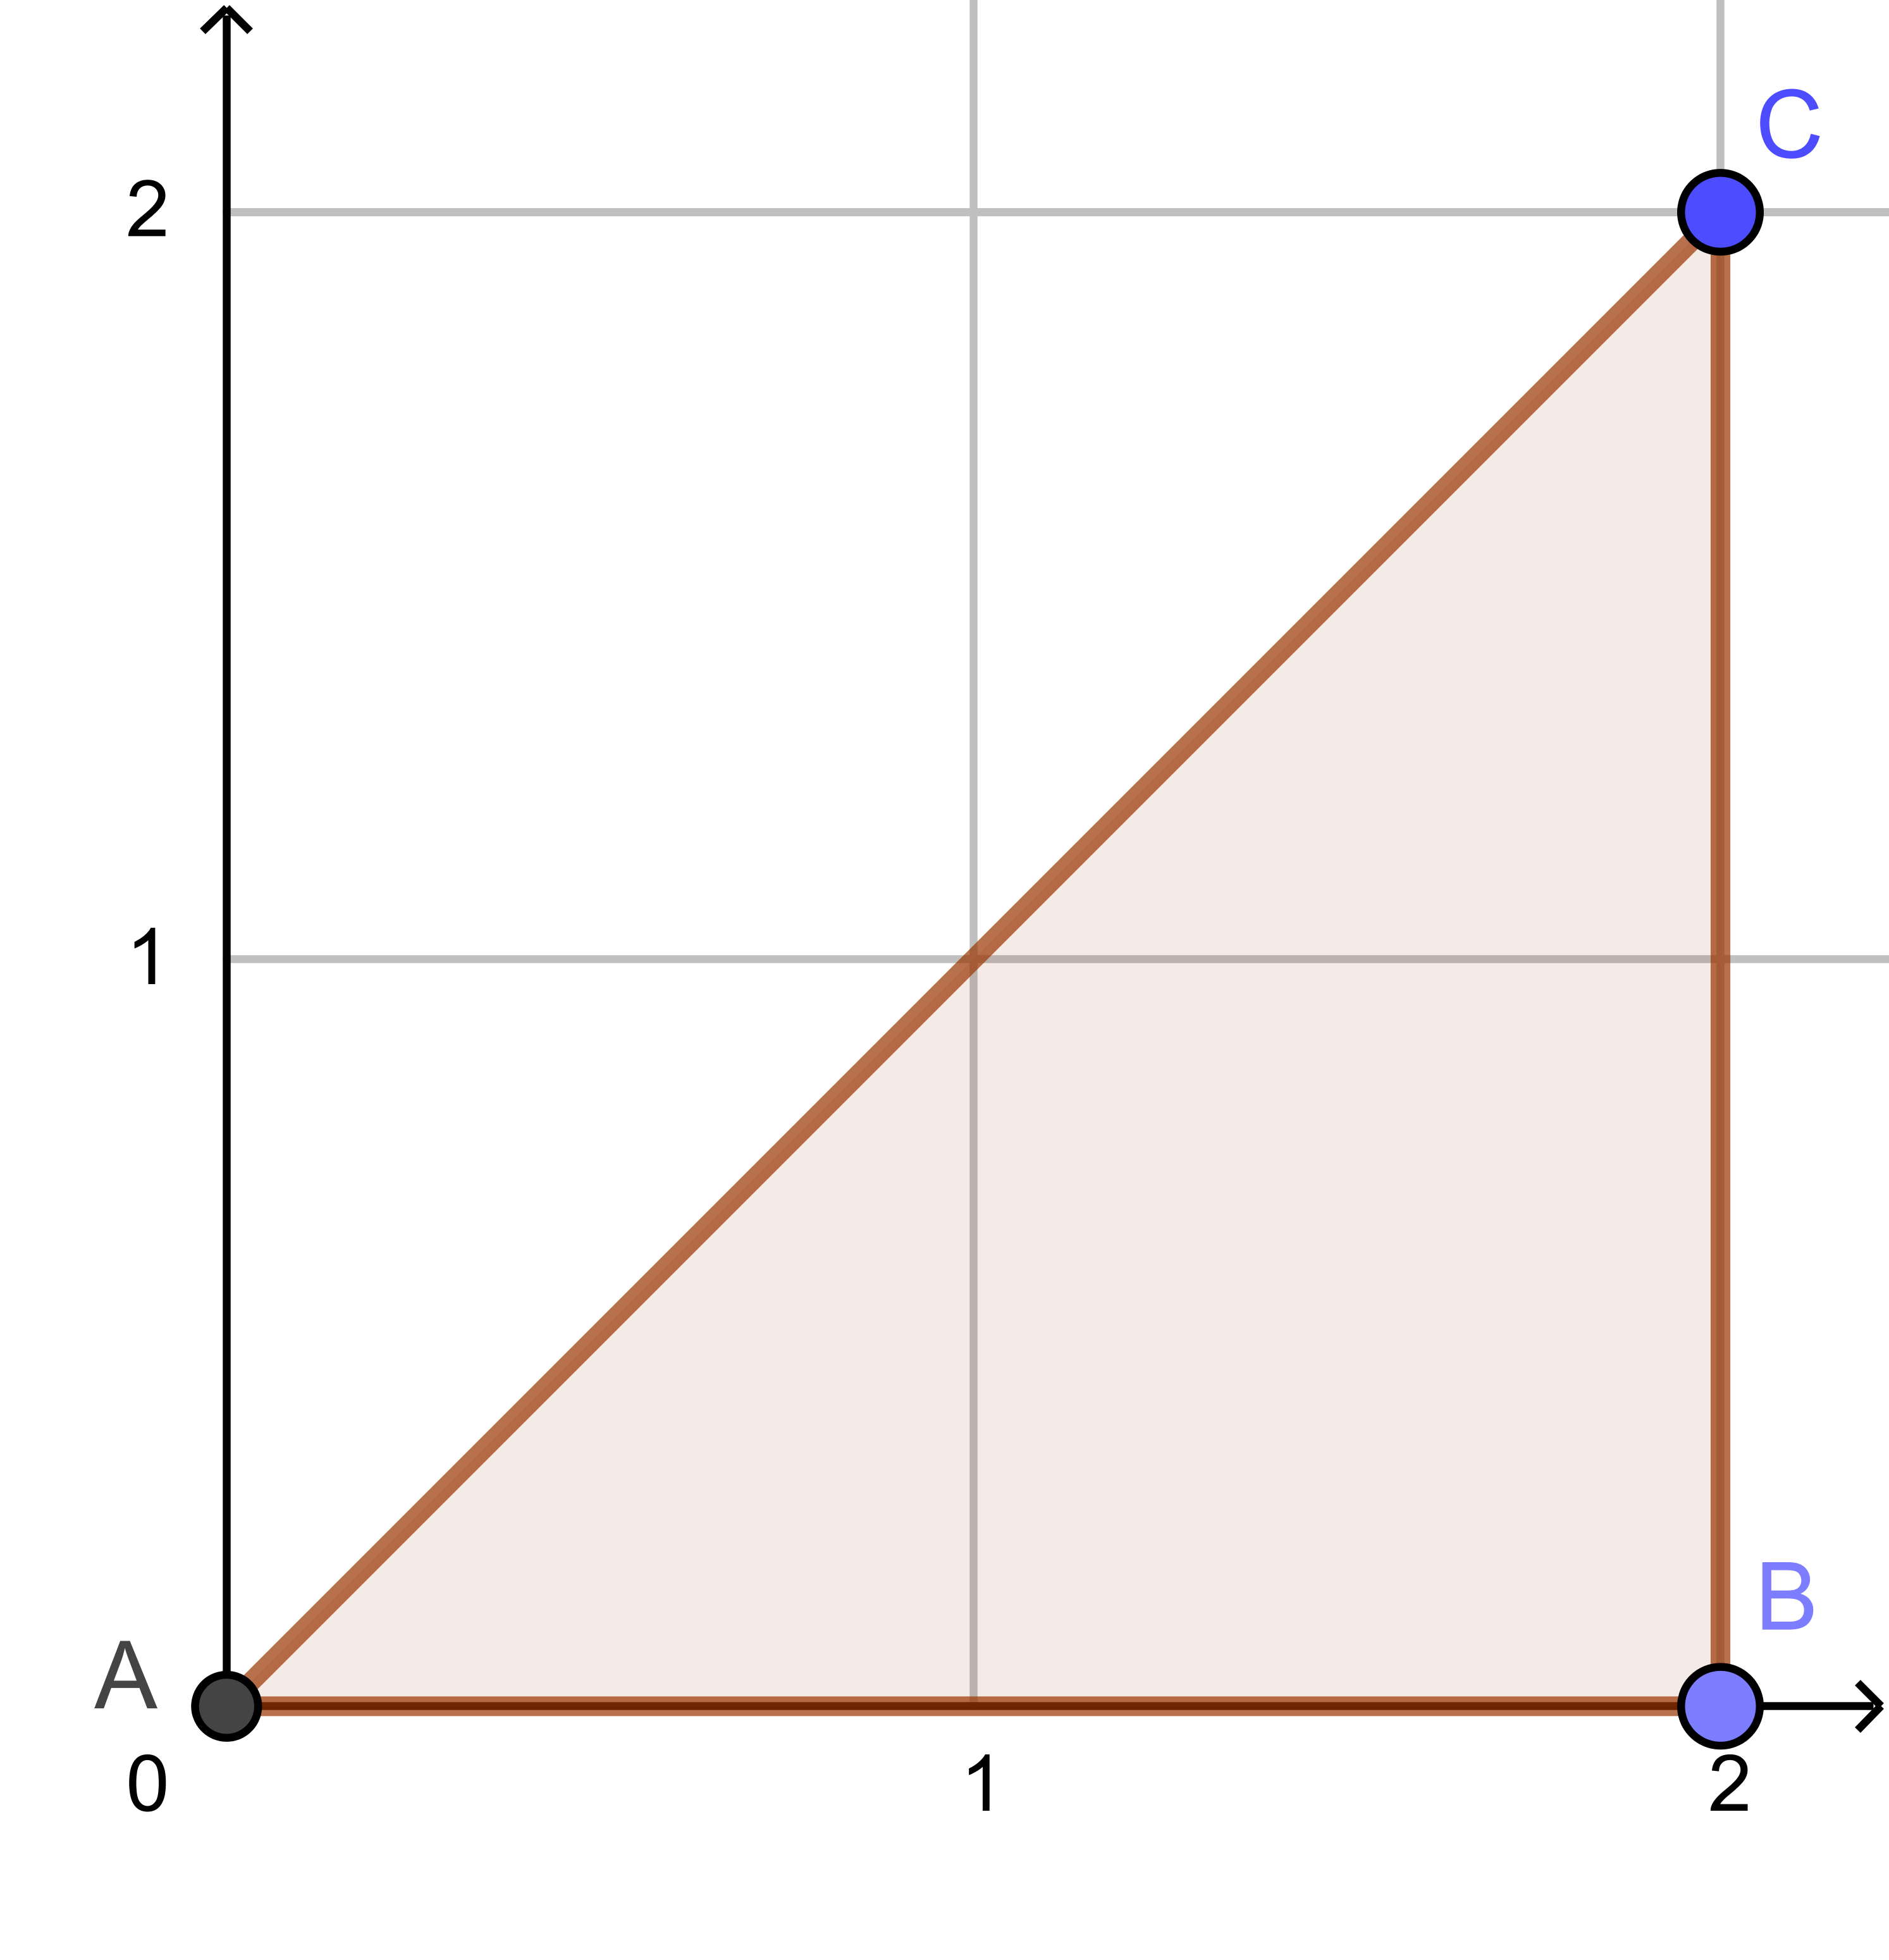
\includegraphics[width=.9\textwidth]{img/2-1-1}
\par\bigskip\uncover<8>{
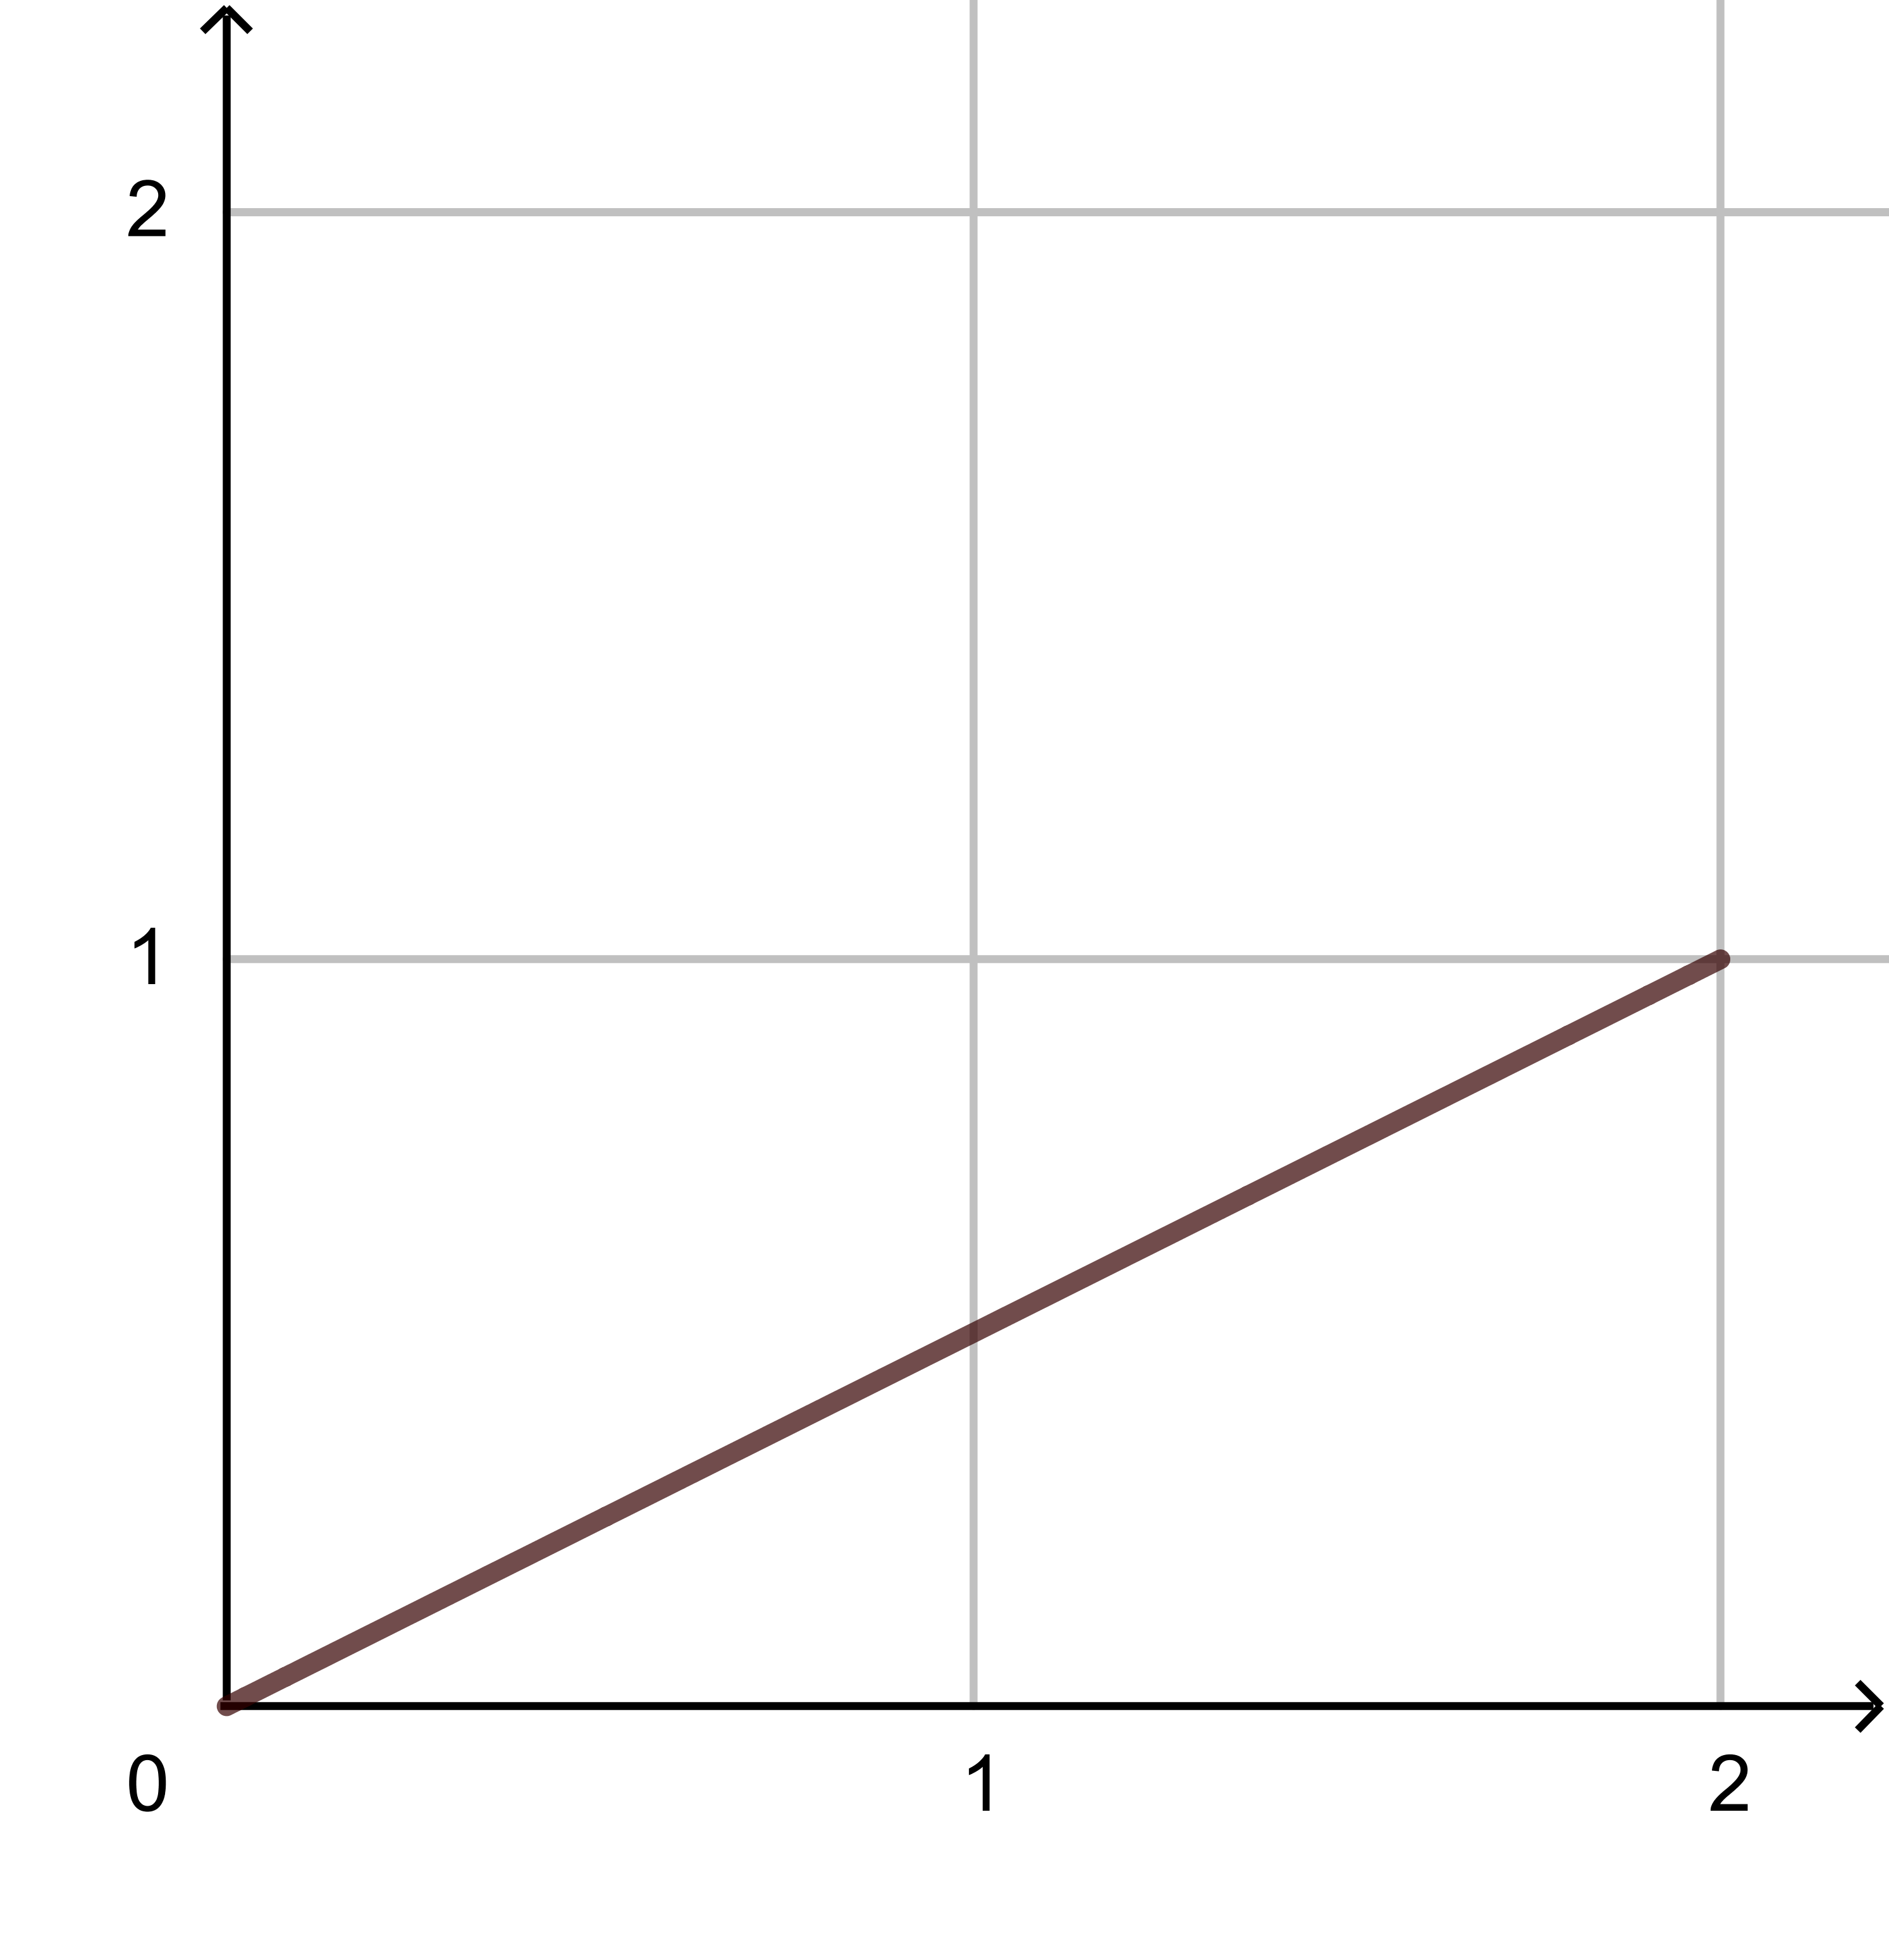
\includegraphics[width=.9\textwidth]{img/2-1-2}}
\end{minipage}
\end{frame}

%%
\begin{frame}[t]{\subsecname}
철수는 12시에서 1시 사이에 아무때나 은행에 방문하기로 하였다.
철수가 은행에 방문한 시각을 12시 \(X\)분이라고 하자.\par
\begin{enumerate}[(1)]
\item<1->
가능한 \(X\)의 값의 범위는 \rb{2-}{0\le X\le 60}이다.\\[5pt]
따라서 \(X\)는 (이산확률변수, {\color<2->{red}{연속확률변수}})이다.
\item<3->
\(P(0\le X\le20)=\rb{4-}{\frac13}\),\qquad
\(P(30\le X\le45)=\rb{4-}{\frac14}\)
\item<5->
\(P(X=20)=\rb{6-}0\),\qquad
\(P(X=45)=\rb{6-}0\)
\end{enumerate}
\par\bigskip
\begin{minipage}{.6\textwidth}
\uncover<7>{
이 경우에도 확률질량함수 \(P(X=x)\)를 생각하는 것이 아무런 의미가 없다.
대신, 확률밀도함수 \(f(x)\)를 고려하는데, 이 함수는 
\[P(a\le X\le b)=\int_a^bf(x)\,dx\]
를 만족시킨다.
이 문제에서 확률밀도함수는 \(f(x)=\frac1{60}\)이다.}
\end{minipage}
\begin{minipage}{.36\textwidth}
\uncover<7>{
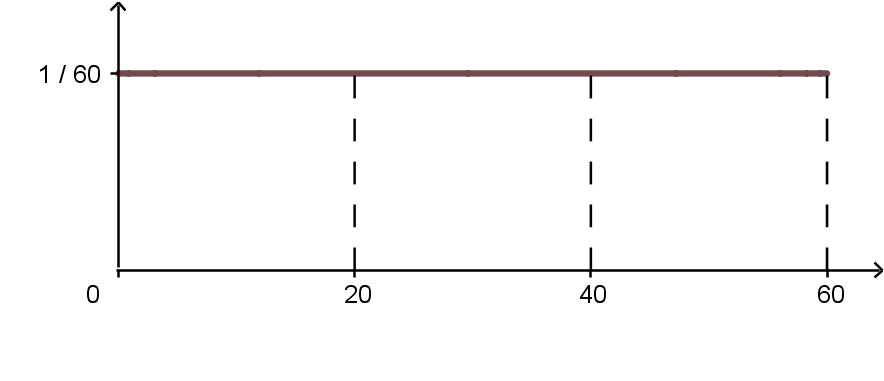
\includegraphics[width=.9\textwidth]{img/2-2-1}}
\end{minipage}
\end{frame}

%%
\begin{frame}[t]{\subsecname}
연속확률변수 \(X\)가 값을 가질 수 있는 범위가 \(\alpha\le X\le \beta\)일 때, 다음 세 가지 성질을 만족시키는 함수 \(f(x)\)를 \(X\)의 \alert{확률밀도함수}라고 한다.\par\bigskip
\begin{minipage}{.48\textwidth}
\begin{itemize}
\setlength{\itemsep}{15pt}
\item
\(f(x)\ge0\)
\item
\(\displaystyle\int_\alpha^\beta f(x)\,dx=1\)
\item
\(\displaystyle\int_a^b f(x)\,dx=P(a\le X\le b)\)
\end{itemize}
\par\bigskip
\begin{center}
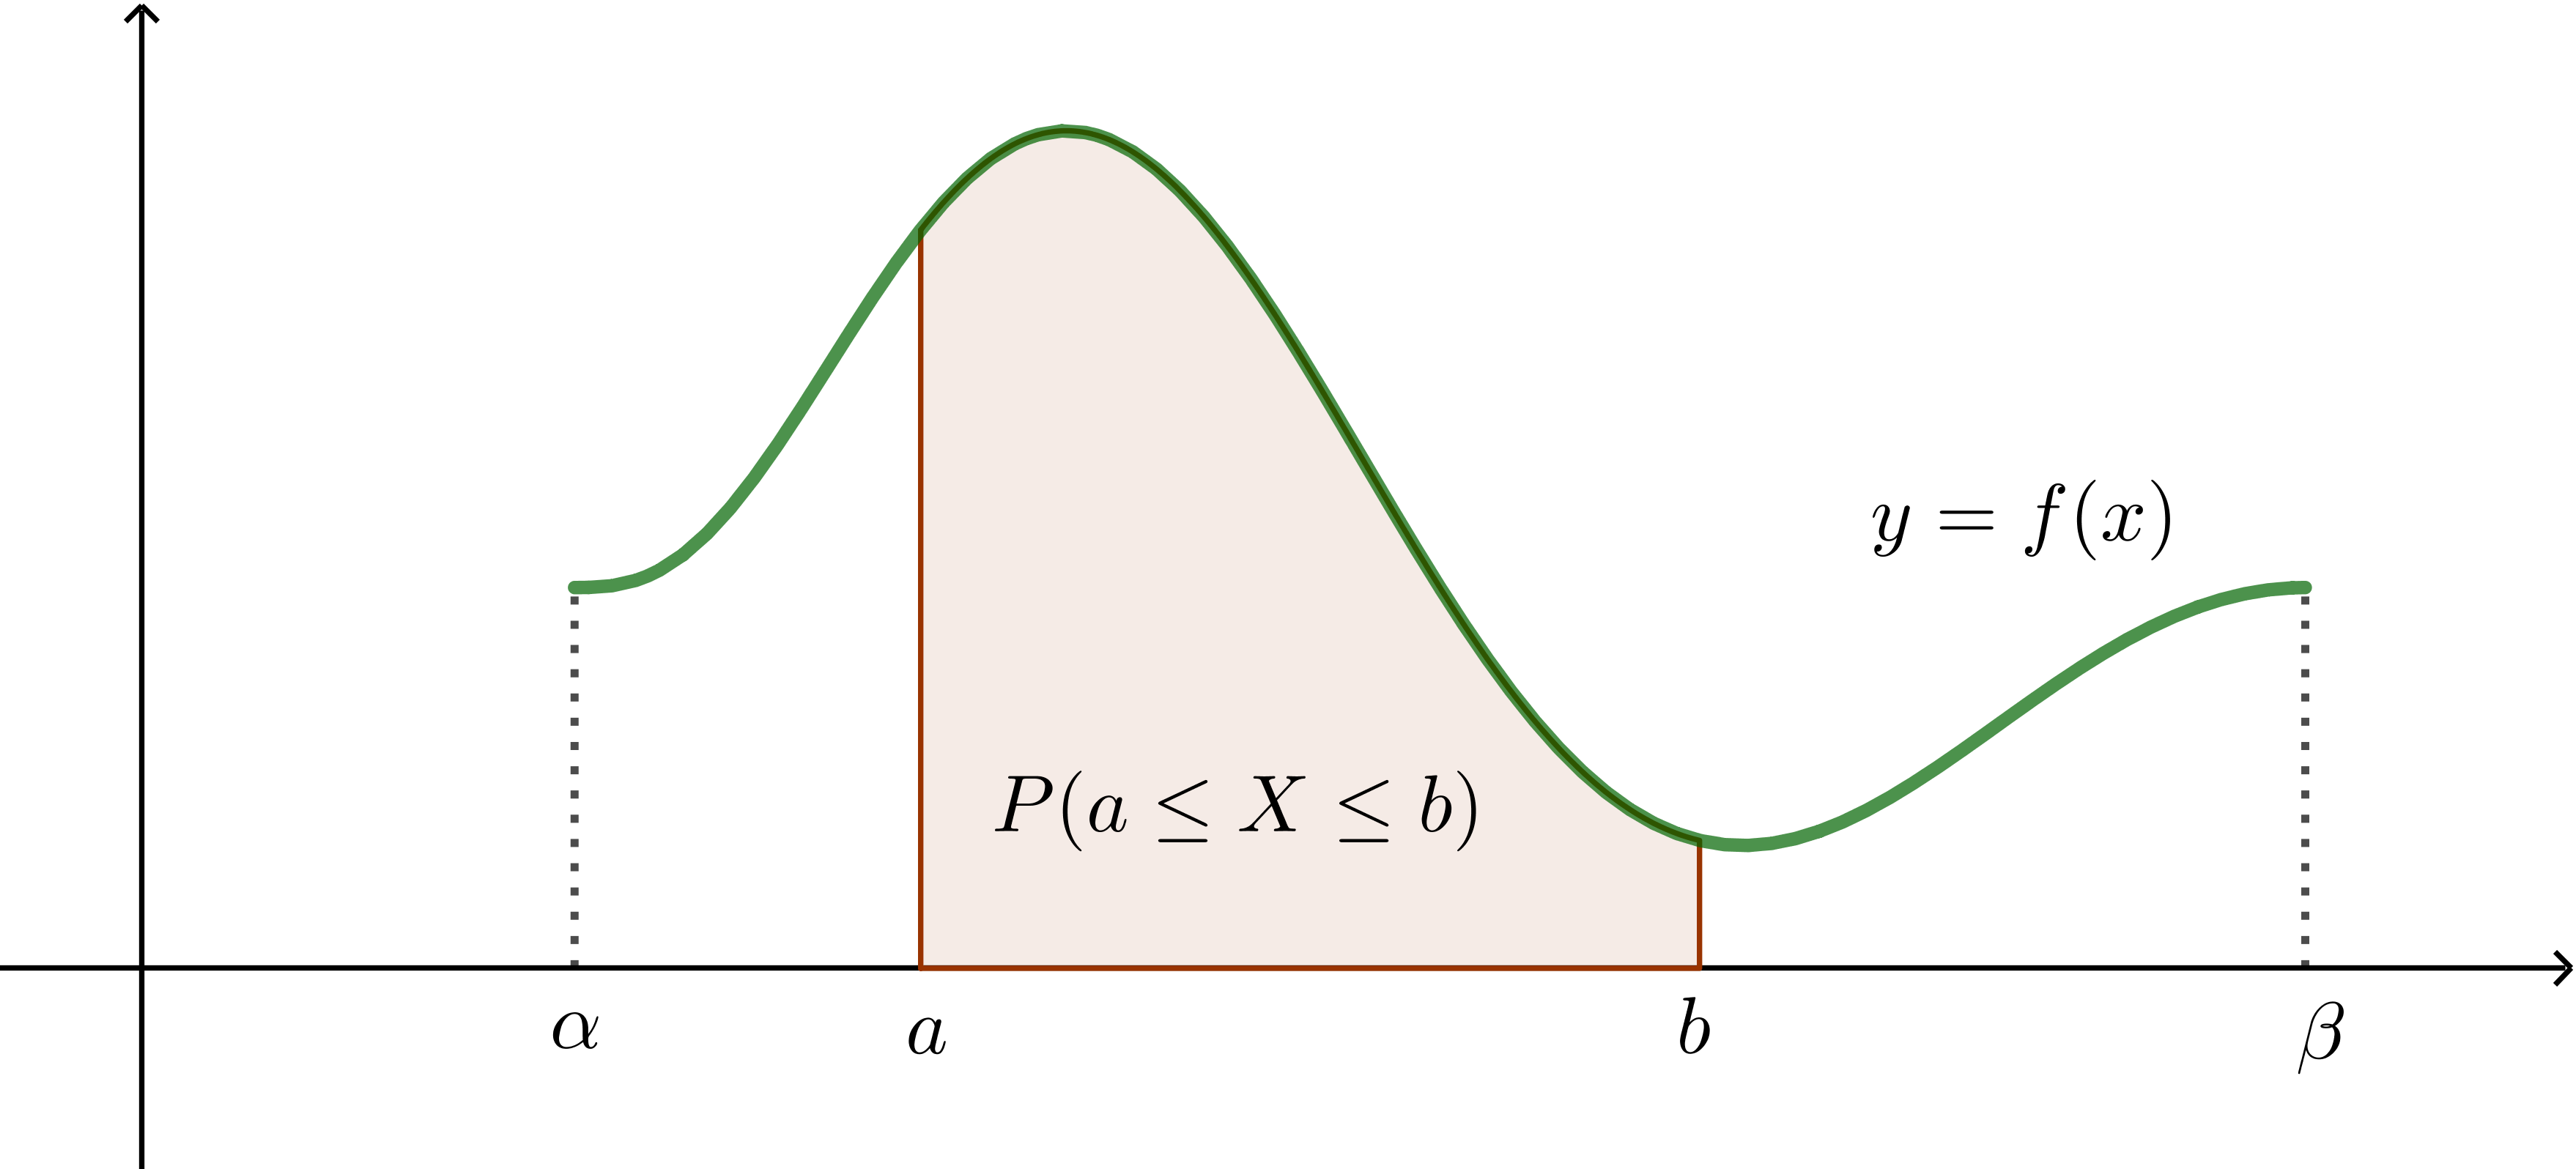
\includegraphics[width=.8\textwidth]{img/2-3-1}
\end{center}
\end{minipage}
\pause
\begin{minipage}{.46\textwidth}
\color{gray}{
\begin{itemize}
\setlength{\itemsep}{15pt}
\item
\(\color{gray}{0\le p_i\le1}\)
\item
\(\color{gray}{\displaystyle\sum_{i=1}^np_i=1}\)
\item
\(\color{gray}{\displaystyle\sum_{i=j}^kp_i=P(x_i\le X\le x_k)}\)
\end{itemize}
\par\bigskip
\begin{center}
\begin{tabularx}{\textwidth}{|N|N|N|N|N|N|}
\hline
\multicolumn2{|>{\centering\setlength\hsize{2\hsize}$}X<{$}|}{X}		&x_1	&x_2	&\cdots	&x_n 	\\\hline
\multicolumn2{|>{\centering\setlength\hsize{2\hsize}$}X<{$}|}{P(X=x_i)}	&p_i	&p_2	&\cdots	&p_n 	\\\hline
\end{tabularx}\end{center}}
\end{minipage}
\end{frame}

%%%
\subsection{정규분포}
%%
\begin{frame}[t]{\subsecname}
\begin{minipage}{.6\textwidth}
%
\begin{exam}{}
어느 고등학교에서 남학생의 키를 \(X\)라고 할 때, \(X\)의 분포가 다음과 같이 생겼다고 한다.
\begin{enumerate}[(1)]
\item
이 고등학교 남학생들의 키의 평균은 \rb2{175}cm 이다.
\item
키가 175cm에서 180cm인 학생들보다는 180cm에서 186cm인 학생들이 더 ({\color<2->{red}{많다}}, 적다).
\end{enumerate}
\end{exam}
\end{minipage}
\begin{minipage}{.37\textwidth}
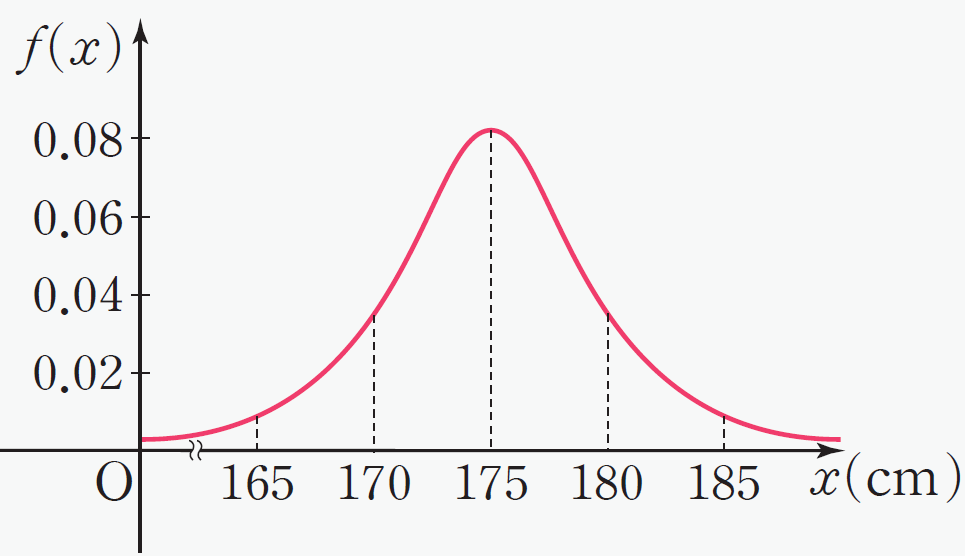
\includegraphics[width=\textwidth]{img/3-1-1}
\end{minipage}
\par\bigskip\pause
%
\begin{defi}{) 정규분포}
사회나 자연에서 일어나는 많은 현상들에서 나타나는 자료들은 위의 그래프처럼 좌우 대칭인 종 모양의 분포를 가지는 경우가 많다.
이와 같은 분포를 \alert{정규분포}라고 한다.
\end{defi}
\bigskip

\begin{minipage}{.6\textwidth}
연속확률변수 \(X\)가 평균이 \(m\)이고 표준편차가 \(\sigma\)인 정규분포를 따를 때 기호로
\[X\sim N(m,\sigma)\]
라고 쓴다.
이때, 확률밀도함수 \(f(x)\)는
\[f(x)=\frac1{\sqrt{2\pi}\sigma}e^{-\frac{(x-m)^2}{2\sigma}}\]
이다.
\end{minipage}
\begin{minipage}{.37\textwidth}
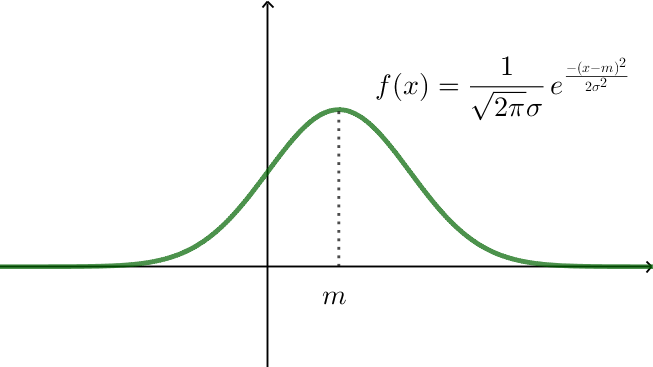
\includegraphics[width=\textwidth]{img/3-2-1}
\end{minipage}
\end{frame}

%%
\begin{frame}[t]{\subsecname}
%
\begin{theo}{) 정규분포 곡선의 성질}
\begin{enumerate}[(1)]
\item
정규분포의 확률밀도함수는 \(x=m\)일 때 최댓값을 가진다.
따라서, 평균 \(m\)이 커질수록 정규분포 곡선은 (왼쪽으로, {\color<2->{red}{오른쪽으로}}) 이동한다.
\item
표준편차 \(\sigma\)는 이 분포가 얼마나 넓게 분포되어 있는지를 나타내는 값이다.
따라서, 표준편차 \(\sigma\)가 커질수록 정규분포 곡선은 ({\color<2->{red}{넓게 퍼진다}}, 뾰족하게 모인다).
\end{enumerate}
\end{theo}
\pause
\begin{minipage}{.45\textwidth}
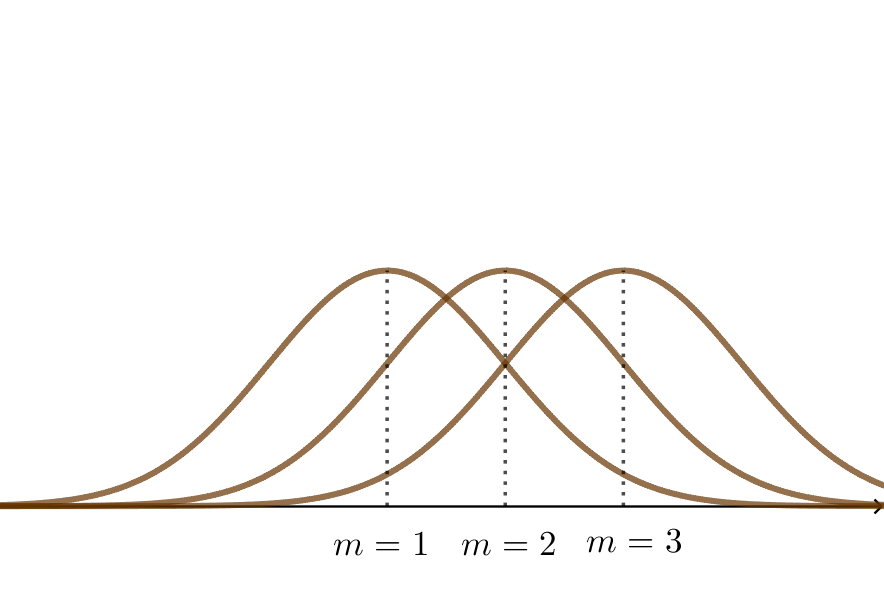
\includegraphics[width=\textwidth]{img/3-3-1}
\end{minipage}~~
\begin{minipage}{.45\textwidth}
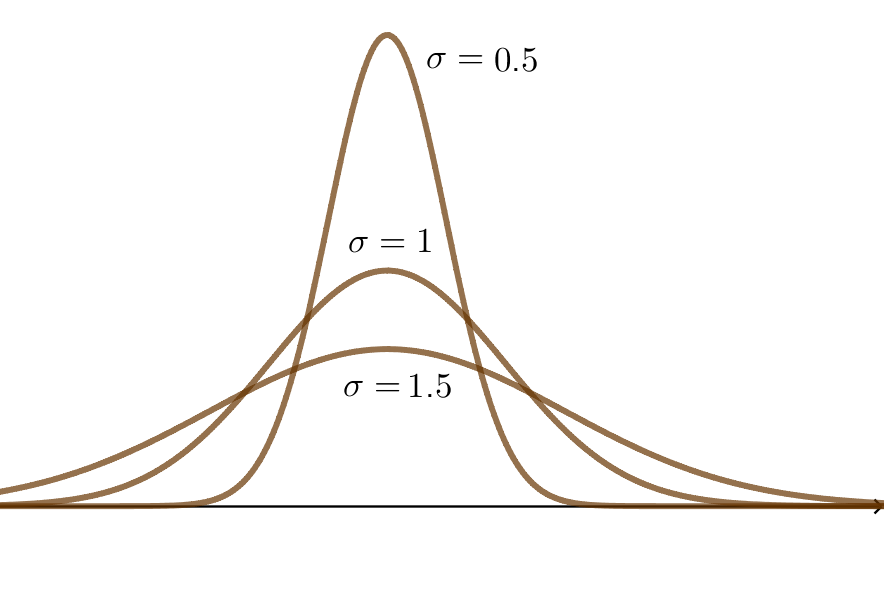
\includegraphics[width=\textwidth]{img/3-3-2}
\end{minipage}
\end{frame}

%%%
\subsection{표준정규분포}
%%
\begin{frame}[t]{\subsecname}
\end{frame}

\end{document}